	

\section{All-order approaches and PYTHIA Monte Carlo generator}

A different approach to describe the phenomena observed at high-energy colliders, instead of calculating cross-sections order by order in the perturbative expansion, is the use of an \textit{all-order} approach. 
\\
%Different all-order approaches exist such as resummation techniques and parton showers. Resummation is based on the observation that in many quantities the smallness of the expansion coefficients $\alpha_s$ is violated by large logarithmic enhancements. This takes the dominant contribution from each order and "resums" them by means of an evolution equation. 
%\\
%The main problem in QCD is related to the fact that lots of quantities have logarithmic corrections that can lead to divergences. Resummation avoids these divergences.
%%The main problem in QCD is related to the fact that lot of quantities have corrections of the form $\alpha_s^n\log^k(Q_i/Q_j)$ where $Q_i$ and $Q_j$ are two different energies scales, for example:
%%\begin{itemize}
%%	\item[--] Renormalization $\mu_R=Q^2$ and factorization scales logs: $\alpha_s^n\log^n(Q^2/\mu_f)$
%%\end{itemize}
%Various methods to perform this resummation exist depending on the process and the type of divergence that has to be eliminated.
%\\
%%%%% GRAPH on pT Z with effect of resummation 
%An example is the $Z$ production $p_T$ spectrum shown in \figRef{figure:pT_Z_CDF}: here the comparison between experimental CDF data and theoretical predictions is shown: in the low $p_T$ region the \textit{all-order} approach regularizes the divergence of the fixed order calculation and describes the data better. 
%
%\begin{figure}[!htb]
%	\centering
%			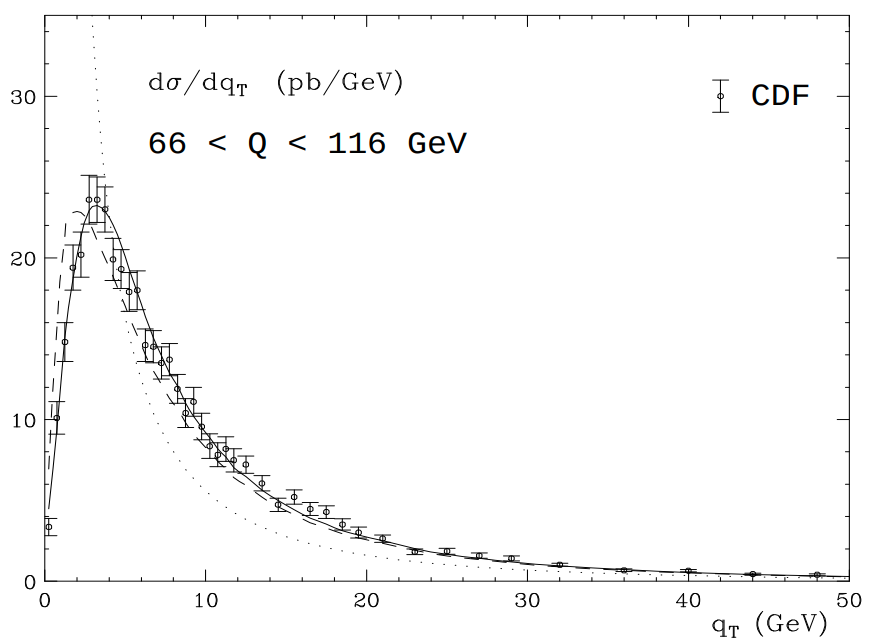
\includegraphics[width=12cm]{{img/pT_Z_CDF.png}}
%	\caption{CDF data on $Z$ production cross-section at Tevatron collider, CDF experiment, the predictions from fixed order calculation (dotted) with resummation (dashed), and with the inclusion of power corrections (solid) are compared. Figure take from \cite{kulesza2002electroweak}}
%	\label{figure:pT_Z_CDF}
%\end{figure}
%
%An other \textit{all-order} approach is based on the simulation of the so-called \textit{parton shower}. It is  implemented in different Monte Carlo programs, as  \textsc{pythia} \cite{PYTHIA2015}, \textsc{herwig} \cite{Herwig2008} and \textsc{sherpa} \cite{SHERPA2004}.
%
%The following sections will focus on parton shower in particular on its implementation in
%\textsc{Pythia}8. \textsc{Pythia} is a standard tool for the simulation of events in high energy collisions. \textsc{Pythia} contains the evolution from a few-body system to a complex multiparticles final state. It simulate a lot of different processes, some of them are described below. Let starts with a discussion on how the parton shower work and how it is implemented in \textsc{pythia}.

The most violent proton-proton collision at the LHC can have a high number of separated jets, $\sim 5\div 10$. If these jets are observed from a nearer point of view what one can observe is a fractal composition of jets-inside-jets-inside-jets. This structure is expected to continue down to the hadronization scale, a bit below $1\ \mathrm{GeV}$. This fractal nature can lead to hundred of partons in the final-state that then are masked inside the hadrons.
The main problem in the theory is that there is no way to perform matrix element calculation to describe such a complicated event topology. Instead, the standard procedure is to use an \textit{all-order} approach: \textit{parton showers}.  




\subsection{Parton Showers}
 
%The idea is to start from the matrix element calculation of the hard interactions and then apply the parton shower to the partons participating in it. The parton shower dress up the partons by emissions at successively "softer" and "more collinear" resolution scales. This shower is build in a recursive manner from the larger scale defined by the hard process toward the cutoff at the hadronization scale.   
 
The parton shower algorithm starts from a few partons arising from a hard interaction evaluated by means of the matrix element calculation. Then, as the energy scale at which the scattering is examined decreases these harder partons can split by emission of gluons or quark anti-quark pairs, and so more partons are produced in the shower that can split in their turn. In this process, the higher scale partons are related to the lower hadronization energy scale (close to $1 \ \mathrm{GeV}$) using the DGLAP evolution equation formalism. The solution to this equation can be written using a \textit{Sudakov form factor} arising from the probability of no gluon emission in the evolution from higher to lower scale and it ensures the unity for the branching total probability.
\\
In the parton showering process, in addition to the kinematic variables (momentum fraction $z$ and azimuthal angle $\phi$) and flavours of the partons, an evolution variable $t$ is generated. \textsc{Pythia8} uses as  evolution variable the squared of the relative transverse momentum of the two partons in the splitting ($p_T^2$). Different choices are made in \textsc{herwig} and \textsc{sherpa}.
\\
As mentioned before, the shower evolution is based on the standard (LO) DGLAP splitting kernels P(z) described here:
\begin{align}
P_{q\,\rightarrow\,qg}(z) & = C_F\frac{1+z^2}{1-z}\quad ; \label{eq:DGLAP_splitting1}\\
P_{g\,\rightarrow\,gg}(z) & = C_A\frac{(1-z(1-z))^2}{z(1-z)}\quad ; \label{eq:DGLAP_splitting2}\\
P_{q\,\rightarrow\,q\overline{q}}(z) & = T_R(z^2+(1-z)^2)\quad ; \label{eq:DGLAP_splitting3}
\end{align} 
where $C_F=\frac{4}{3}$ is the Casimir operator for $SU(3)$, $C_A=N_C=3$, that are named "color factors", and $T_R=\frac{1}{2}$ that is given by the trace calculation of the group generators, each contribution is multiplied by $N_f$ if summing over all contributing quark flavours.
\\
The parton shower consists of two components: the initial-state radiation describing the emission from the incoming partons and the final-state radiation describing the emission of outgoing partons they are also respectively referred to as spacelike and timelike showers.
Both ISR and FSR algorithms are based on these splitting kernels introduced in \eqRef{eq:DGLAP_splitting1}, \ref{eq:DGLAP_splitting2} and \ref{eq:DGLAP_splitting3}.
The respective probabilities of emitting radiation as one move in the decreasing evolution variable sequence are:
\begin{align}
	FSR: \qquad\quad & \frac{d\mathcal{P}_{FSR}}{dp_T^2} = \frac{1}{p_T^2}\displaystyle\int \frac{dz}{z}\,\frac{\alpha_s}{2\pi}P(z)\quad ;\label{eq:FSR1}\\
	ISR: \qquad\quad & \frac{d\mathcal{P}_{ISR}}{dp_T^2} = \frac{1}{p_T^2}\displaystyle\int \frac{dz}{z}\,\frac{\alpha_s}{2\pi}P(z)\,\frac{f'(x/z,p_T^2)}{f(x,p_T^2)}\quad .\label{eq:ISR1}
\end{align}
Where the FSR one represents the infinitesimal probability that a parton branches, or in this case decays, in a $dp_T^2$ step.
Instead, \eqRef{eq:ISR1} refers to the same probability but it includes the description of the PDF evolution in fact the ISR is described in terms of production of a parton (instead of decays probability as in FSR). The slitting kernels are the same described above except that the splitting probability for the  production of a gluon is equal to $2P_{g\,\rightarrow\,gg}(z)$ since two gluons are generated from the decay of one gluon.

Staring from these infinitesimal probabilities by multiplication of no-emission probability $1-dP_{ISR}$, or equally $1-dP_{FSR}$. 
The Sudakov form factor can be written as: % by means of the two probability in \eqRef{eq:FSR1} and \eqRef{eq:ISR1}, as
\begin{equation}
	\Delta(p_T^2)=\exp\left( -\displaystyle\int_{p_{T0}^{PS}}^{p_T'} \frac{d\mathcal{P}_{PS}}{dp_T^2} \,dp_T\right) \qquad\text{ with } \quad PS=ISR,\ FSR \quad.
	\label{eq:sudakovFormFactor}
\end{equation}
The Sudakov form factor gives the probability of a parton to evolve from an harder scale to a softer scale without emitting a parton harder than some resolution scale.
\\
The introduction of the Sudakov form factor resumes all the effects from the soft and collinear gluon emission. For more details and some plots of different Sudakov form factors values see section 3.5 of \cite{Campbell2006}.
\\
The Sudakov factor allows to write the parton shower algorithm using a Markov Chain Monte Carlo method. In fact the system status at a certain value of $p_T$ depends only on the previous status of the system at a $p_T'>p_T$\footnote{It is important to remember that the simulation is described in a downward evolution in the evolution variable, $p_T$. So the previous state of the system is located at a higher value of this variable.}. 
\\
In \textsc{pythia}8 the contributions from ISR and FSR are interleaved into a single common sequence of decreasing $p_T$. 
\\
It has been seen that the solution to the DGLAP equation is given by putting \eqRef{eq:FSR1} and \eqRef{eq:ISR1} in \eqRef{eq:sudakovFormFactor} respectively for the ISR and the FSR by a Sudakov form factor that is related to the no-emission probability in the $p_T$-evolution. 
\\
The evolution variables for ISR and FSR are defined starting from the virtuality ($Q^2$) of the emission:
\begin{equation}
	p_T^2=\left\{\begin{aligned}
		&(1-z)Q^2 && ISR\\
		&z(1-z)Q^2 && FSR
	\end{aligned}\right.\quad,
	\label{eq:partonShowerEvolutionVariables}
\end{equation}
so, in the two cases: for the FSR $Q^2_{FSR}=(p^2-m_0^2)$ a time-like virtuality ($p^2>0$) is implicated corresponding to a forwards evolution, while for the ISR one has $Q^2_{ISR}=(-p^2+m_0^2)$ with a space-like virtuality ($p^2<0$) describing the backwards evolution. In both cases $Q^2$ values are positively defined. 

%Then the actual strong of the radiation is set by the choices of $\alpha_{s\,ISR}$ and $\alpha_{s\,FSR}$ values.

\noindent The two cutoffs on the transverse momentum scale for ISR, $p_{T0}^{ISR}$, and FSR, $p_{T0}^{FSR}$,  are free parameters in \textsc{pyhtia} and are called \texttt{Space}\-\texttt{Shower:}\-\texttt{pT0}\-\texttt{Ref}   and \texttt{Time}\-\texttt{Shower:}\-\texttt{pT0}\-\texttt{min}.

\medskip

The parton showers alone are certainly not the whole story in describing the exclusive structure of an event. They are based on collinear and soft approximation. A good description of the hard wide-angle emission and multi-jet final-states cannot be ignored in order to describe many of the observables of interest. So, it is important to perform an higher-order matrix element calculations to describe better all these observables.  


\subsection{Merging parton showers and NLO matrix element calculations}
\label{sec:merging}

Regions dominated by soft and collinear gluon emissions are described very well by parton showers approach; on the other hand, regions, where partons are  energetic and widely separated, are well described by matrix element calculations and not by parton showers.  
So, the best approach would be to combine the two different descriptions, and this is what is performed in the Monte Carlo generators. But to combine NLO matrix element calculation with parton showers the naive procedure of simply adding a parton shower to an event generated with a matrix element generator does not work.
\\
One problem arises from the fact that tree-level matrix elements are \textit{inclusive}, i.e. they give the probability of having at least $n$ partons in a state calculated exactly to the lowest order in $\alpha_s$, while the corresponding state generated by a parton shower is \textit{exclusive}, i.e. gives the probability that there are exactly $n$ partons calculated approximately to all orders in $\alpha_s$
\\
The second problem is to avoid the \textit{double-counting} of some regions of phase space or, conversely, the undercount other regions.
\\
To solve these problems there are different strategies. The various strategies are divided into two groups. The ones referred to as \textit{"match"} are those approaches in which high-order corrections to an inclusive process are integrated with the parton shower. The other strategy involves a \textit{"merge"} this is done by defining a merging scale, where any parton produced above that scale is generated with a corresponding higher-order matrix element and any parton produced below is generated by the shower.
\\
An example of merging approach is the FxFx merging scheme, developed by Frixione, Nason, Webber in the \textsc{mc@nlo} framework \cite{FxFx1,FxFx2,FxFx3,FxFx4}. In this scenario the risk of  double counting is given by the fact that at NLO one emission can be made explicit as indicated in \figRef{fig:DoubleCounting} by the red gluon line, and  then the progress of the parton shower can leads to a double counting between real emission matrix element and the parton shower as shown in \figRef{fig:DoubleCounting}, the double-counting sources are indicated by the blue arrows.
% TODO: mi piacerebbe aggiungere una descrizione più completa del merging con FxFx visto che viene usato dopo. 

%%%
%%% Immagine di Frixi.. presentation
\begin{figure}[H]
	\centering
	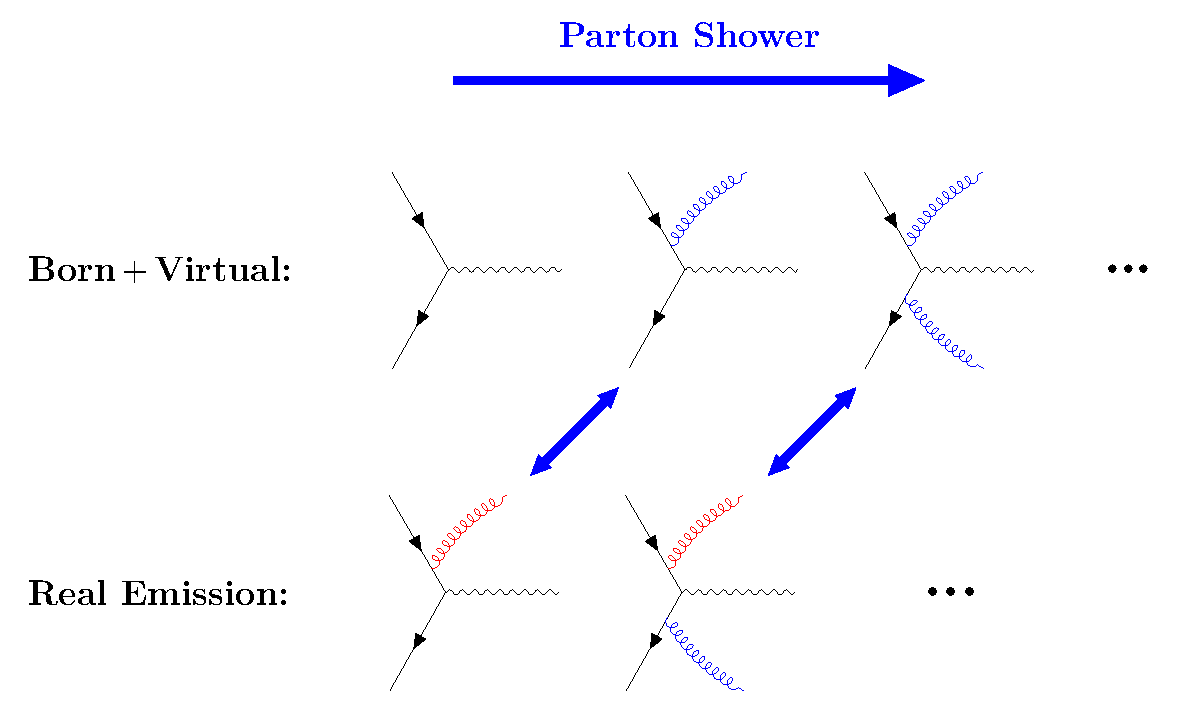
\includegraphics[width=12cm]{{img/feynman_doubleCounting_FxFx_curved-cropped.pdf}}
	%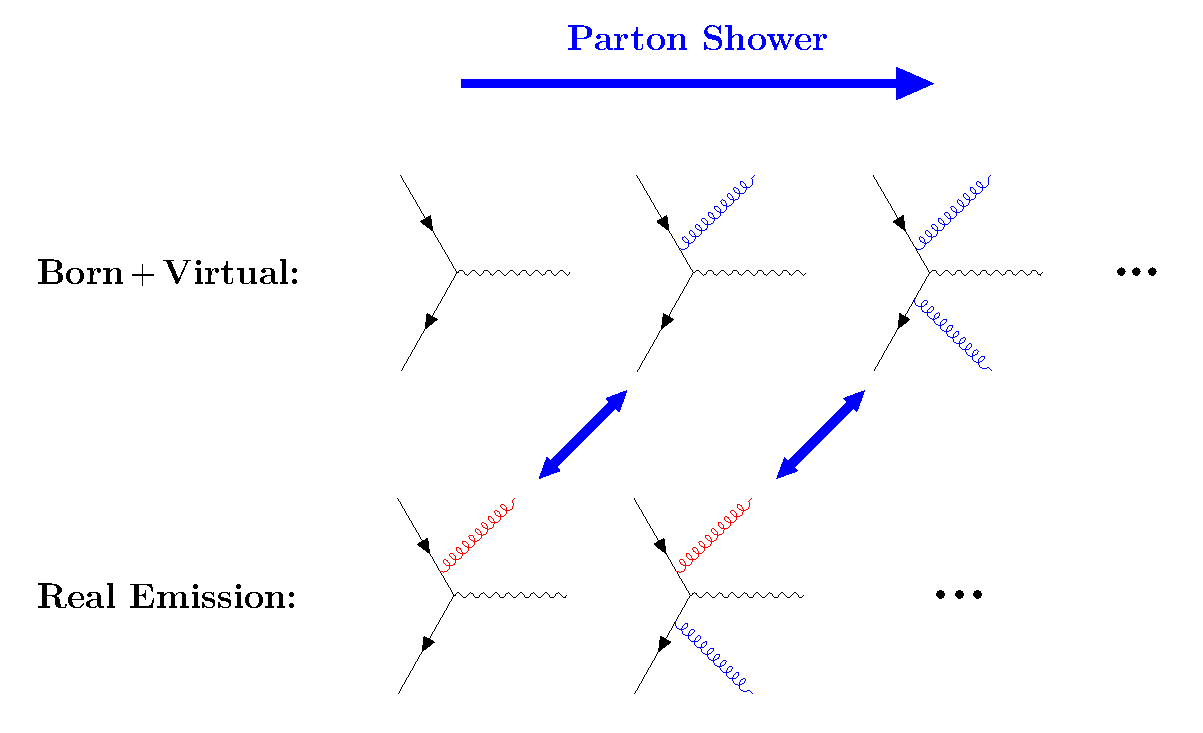
\includegraphics[width=14cm]{{img/feynman_doubleCounting_FxFx-cropped.pdf}}
	\caption{The FxFx margin scheme have to avoid this double counting. Feynman diagrams that can lead to a double counting are grouped with a blue arrow, the blue emission are related to the parton shower while the red ones to the NLO process.}
	\label{fig:DoubleCounting}
\end{figure}
%%%

\noindent So, it is clear that the matrix element calculations cannot be blindly combined with parton showers. The combination of these two approaches is a very active research topic, and is important for giving
a good description for jet production from QCD.


%%%% AGGIUNTA
\section{Soft QCD processes}


Lots of physics processes and modeling issues are related to as "soft QCD". In the following, firstly, is performed a brief introduction of different QCD processes that form the dominant part of the total hadron-hadron cross-section. Then, the model of the Multi Parton Interaction and its implementation in pyhtia8 are described. Lastly, the primordial $k_T$ concept, the color reconnection and the hadronization processes are introduced. All these contributions have to be understood if one wants to have a good description of the soft QCD contribution to what is observed, in particular for the description of the UE.

\subsection{Various contributions to hadron-hadron cross-section}

Hadron-hadron scatterings are classified by the characteristics of the final states. The main division is between \textit{elastic} and \textit{inelastic} scatterings. In elastic ones:
\begin{equation}
	A(p_A)+B(p_B)\ \longrightarrow \ A(p_A')+B(p_B') \quad,
\end{equation} 
both the hadrons $A$ and $B$ emerge intact and no other particles are produced. The only exchanged quantity is momentum. \figRef{fig:CS-elastic} shows how the topology of an observed elastic event would be.

\begin{figure}[!htb]
	\centering
	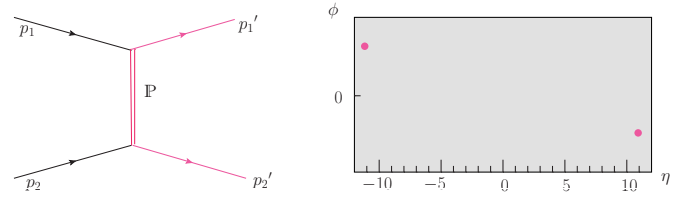
\includegraphics[width=10cm]{{img/CS-elastic.png}}
	\caption{Elastic scattering diagram and $\phi$-$\eta$ plot showing the angular  distribution of products after the interaction. Figure from \cite{DiffractionInPythia}}
	\label{fig:CS-elastic}
\end{figure}

\noindent All the other cases are classified as inelastic. In inelastic scatterings the final-state is different from the initial one.
\begin{equation}
	A(p_A)+B(p_B)\ \longrightarrow \ X\quad.
\end{equation} 
Where $X$ indicates that a new final state has been generated in the interaction. In this case, the system gets complex and new particles are produced. 
\\
So, the total cross-section can be written-out as a sum of two contributions:
\begin{equation}
	\sigma_{\text{tot}}(s) = \sigma_{\text{el}}(s) + \sigma_{\text{inel}}(s)\quad.
	\label{eq:cross_section_elastic_inelastic}
\end{equation}
Where the various contribution depend on the center-of-mass energy squared $s=(p_A+p_B)^2$.
\\
The inelastic contribution can be further subdivide into \textit{diffractive} and \textit{non-diffractive} events. The division is based on the presence, or not, of a large rapidity gap somewhere in the final-state that can be seen as a decay of an excitation of the beam particles.

\subsection{Diffractive cross-section} 

Once an event has been classified as diffractive it is possible to distinguish between three possible classes of diffractive events: \textit{double-diffractive} (DD), \textit{single-diffractive} (SD) and \textit{central-diffractive} (CD). 
In DD events both the particles of the beams are excited and both are fragmented in the collision (\figRef{fig:NONdif_CD_DD_SD}b), on the other hand in SD dissociation just one of the two hadrons get excited while the other survives the collision intact (\figRef{fig:NONdif_CD_DD_SD}a). In the last case, CD, both the beam particles survive intact, but they leave an excited state in the central region that then decays (\figRef{fig:NONdif_CD_DD_SD}c).
\\
So, the inelastic cross-section in \eqRef{eq:cross_section_elastic_inelastic} can be rewritten as:
\begin{equation}
	\sigma_{\text{inel}}(s) = \sigma_{\text{SD}}(s)+\sigma_{\text{DD}}(s)+\sigma_{\text{CD}}(s)+\sigma_{\text{ND}}(s)  \quad,
\end{equation}
where ND are all the \textit{non-diffractive} inelastic events\footnote{It has to be mentioned that other topologies are possible defined as multi-diffractive events whit various  rapidity gap observed. These types of events have a very low cross-section ($\ll 1 \ \mathrm{mb}$) with respect to the other considered.} (\figRef{fig:NONdif_CD_DD_SD}d), these types of events are the dominants in proton-proton collisions at LHC.

\begin{figure}[!htb]
	\centering
	\noindent
	\begin{subfigure}{0.5\textwidth}
		\centering
		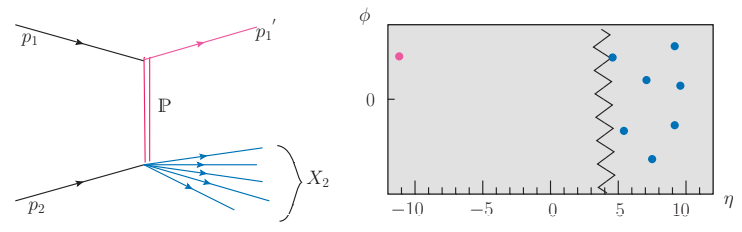
\includegraphics[width=\textwidth]{{img/CS-SD.png}}
		\caption*{a)}
	\end{subfigure}%
	\begin{subfigure}{0.5\textwidth}
		\centering
		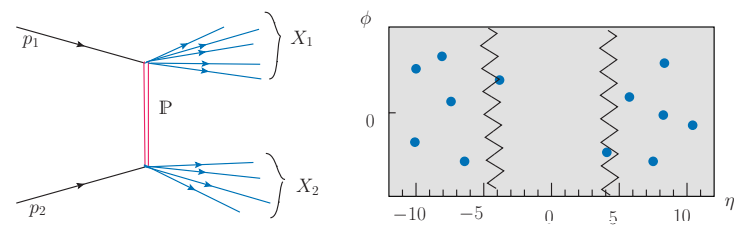
\includegraphics[width=\textwidth]{{img/CS-DD.png}}
		\caption*{b)}
	\end{subfigure}\\[20pt]
	\begin{subfigure}{0.5\textwidth}
		\centering
		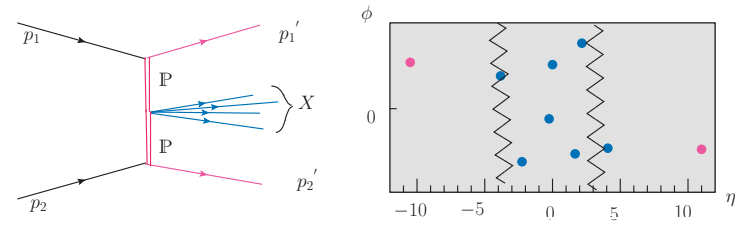
\includegraphics[width=\textwidth]{{img/CS-CD.png}}
		\caption*{c)}
	\end{subfigure}%
	\begin{subfigure}{0.5\textwidth}
		\centering
		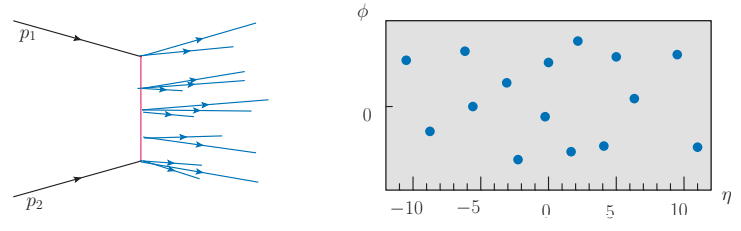
\includegraphics[width=\textwidth]{{img/CS-ND.png}}
		\caption*{d)}
	\end{subfigure}
	\caption{The figure shows: a) an SD event with a rapidity gap in the region $-10<\eta<3.5$; b) a DD event where all the two hadrons fragment and is formed a rapidity gap $|\eta|<3.5$; c) the two hadrons survive but a central excitation is produced (CD event); d) an ND event all the $\phi-\eta$ region is covered by the products of the collision. Figure from \cite{DiffractionInPythia}}
	\label{fig:NONdif_CD_DD_SD}
\end{figure}

The next section will focus on the description of the non-diffractive part of the total cross-section using the MPI model. In very rough terms, this means that the non-diffractive cross-section is saturated by more than a single partonic scattering and that the number of partonic interactions is determined by a Poisson distribution. This model has been very successful in the description of many experimental measurements at hadron colliders.

\section{Multiple Parton Interactions in PYTHIA}


Since hadrons can be viewed as "bunches" of partons, it is likely that in the same hadron-hadron collision more than one pair of partons can undergo to a scattering. This phenomenon is known as \textit{Multiple Parton Interactions} and is related to the composite nature of the incoming hadrons. 
\\
So, it is clear that at some level these MPI have to exist, and they can become important in the description of the event; they can change the color topology of the colliding system as a whole.  
\\
In this scenario, it is important to have a good understanding of the phenomenon. The aim of this section is to describe the basic concepts that are used to simulate MPI, for example in \textsc{Pythia} Monte Carlo event generator; then some focus is given to the free parameters that will be tuned in the following sections.

\subsection{Basic Concepts}
\label{sec:BasicConcepts}

The main hypothesis of the MPI model is the validity of the QCD factorization theorem not only for the hard process but also for the other partons scatters.
\\
So, one can write the following formula for the interaction differential cross-section for the hadron-hadron collisions:
\begin{equation}
	\frac{d\sigma_{\text{int}}}{dp_T}=\displaystyle\sum_{i,j,k,l}\displaystyle\int dx_1 \displaystyle\int dx_2 \displaystyle\int d\hat{t}\, f_i(x_1,Q^2)f_j(x_2,Q^2)\frac{d\hat{\sigma}_{ij\,\rightarrow\,kl}}{d\hat{t}}\delta\left( p_\perp^2-\frac{\hat{t}\hat{u}}{\hat{s}} \right) \quad ,
	\label{eq:sigma_int1}
\end{equation}
%This represent the interaction differential cross-section for the hadron-hadron collisions, 
where $\frac{d\hat{\sigma}_{ij\,\rightarrow\,kl}}{d\hat{t}}$ is the differential cross-section for QCD hard $2\ \rightarrow 2$ processes, this processes are the one reported in \tableRef{table:partonic_cross_sections}. 
\\
In \eqRef{eq:sigma_int1} the Mandelstam variables associated with the partonic system are used. They are defined as:
\begin{align}
	&\hat{s}=(p_1+p_2)^2=(p_3+p_4)^2=x_1x_2s\\
	&\hat{t}=(p_1-p_3)^2=(p_2-p_4)^2\\
	&\hat{u}=(p_1-p_4)^2=(p_2-p_3)^2
\end{align} 
where $p_1$, $p_2$ are the four-momenta of the incoming partons and $p_3$, $p_4$ the four-momenta of the outgoing partons. 

%Note that in \eqRef{eq:sigma_int1} the jet cross-section is twice as large $\sigma_{\text{jet}}=2\sigma_{\text{int}}$, because at first approximation each interaction gives rise to two jets.

\noindent It has been assumed also that the "hardness" of a  process is defined by the $p_T$ scale of the interaction ($Q^2=p_T^2$).

%\begin{table}[!ht]
%	\centering
%	\begin{tabular}{l | c}\rule{0pt}{3ex} 
%	Process & Partonic cross-section \rule{0pt}{3.5ex}\\   \hline\hline 
%	$q\,q'\ \rightarrow\ q\,q'$ & $\frac{4}{9}\frac{\hat{s}^2+\hat{u}^2}{\hat{t}^2}$\rule{0pt}{3.5ex}\\
%	$q\,q\ \rightarrow\ q\,q$ & $\frac{4}{9}\left(\frac{\hat{s}^2+\hat{u}^2}{\hat{t}^2}+\frac{\hat{s}^2+\hat{t}^2}{\hat{u}^2}\right) -\frac{8}{27}\frac{\hat{s}^2}{\hat{u}\hat{t}}$\rule{0pt}{3.5ex}\\
%	$q\,\overline{q}\ \rightarrow\ q'\,\overline{q}'$ & $\frac{4}{9}\frac{\hat{s}^2+\hat{u}^2}{\hat{t}^2}$\rule{0pt}{3.5ex}\\
%	$q\,\overline{q}\ \rightarrow\ q\,\overline{q}$ & $\frac{4}{9}\left(\frac{\hat{s}^2+\hat{u}^2}{\hat{t}^2}+\frac{\hat{t}^2+\hat{u}^2}{\hat{s}^2}\right) -\frac{8}{27}\frac{\hat{u}^2}{\hat{s}\hat{t}}$\rule{0pt}{3.5ex}\\
%	$q\,\overline{q}\ \rightarrow\ g\,g$ & $\frac{32}{27}\frac{\hat{t}^2+\hat{u}^2}{\hat{t}\hat{u}}-\frac{8}{3}\frac{\hat{t}^2+\hat{u}^2}{\hat{s}^2}$\rule{0pt}{3.5ex}\\
%	$g\,g\ \rightarrow\ q\,\overline{q}$ & $\frac{1}{6}\frac{\hat{t}^2+\hat{u}^2}{\hat{t}\hat{u}}-\frac{8}{3}\frac{\hat{t}^2+\hat{u}^2}{\hat{s}^2}$\rule{0pt}{3.5ex}\\
%	$g\,q\ \rightarrow\ g\,q$ & $-\frac{4}{9}\frac{\hat{s}^2+\hat{u}^2}{\hat{s}\hat{u}}-\frac{\hat{u}^2+\hat{s}^2}{\hat{t}^2}$\rule{0pt}{3.5ex}\\
%	$g\,g\ \rightarrow\ g\,g$ & $\frac{9}{2}\left( 3-\frac{\hat{t}\hat{u}}{\hat{s}^2} -\frac{\hat{s}\hat{u}}{\hat{t}^2} - \frac{\hat{s}\hat{t}}{\hat{u}^2} \right)$\rule{0pt}{3.5ex}
%	\end{tabular}
%	\caption{Parton-Parton differential cross-sections ($2\ \rightarrow\ 2$ QCD process), can beh calculated in pQCD evaluating the matrix element for each process involving quark, antiquark and gluon.}
%	\label{table:partonic_cross_sections}
%\end{table}

\begin{table}[!ht]
	\centering	
	\begin{tabular}{| c | P{6cm} | c |}
	\hline
	Process & Amplitude & $\displaystyle\sum|\mathcal{M}|^2/(4\pi\alpha_s)^2$\\\hline\hline
	$qq'\,\rightarrow\,qq' $ & \scalebox{0.95}{\raisebox{-.5\height}{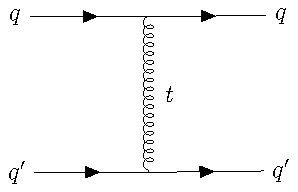
\includegraphics[width=2.5cm]{{img/DiagrammiPartonic/feynman_partonic_1.pdf}}}} & $\displaystyle{ \frac{4}{9}\frac{s^2+u^2}{t^2} }$\\\hline
	$qq\,\rightarrow\,qq $ & \scalebox{0.95}{\raisebox{-.5\height}{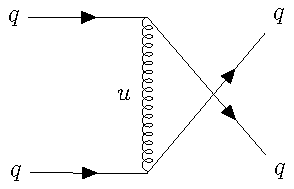
\includegraphics[width=2.5cm]{{img/DiagrammiPartonic/feynman_partonic_2.pdf}}\qquad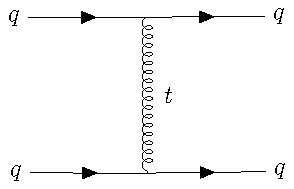
\includegraphics[width=2.5cm]{{img/DiagrammiPartonic/feynman_partonic_3.pdf}}}} & $\displaystyle{\frac{4}{9}\frac{s^2+u^2}{t^2} + \frac{4}{9}\frac{s^2+t^2}{u^2} - \frac{8}{27}\frac{s^2}{tu}}$\\\hline
	$q\overline{q}\,\rightarrow\,q'\overline{q'} $ & \scalebox{0.95}{\raisebox{-.5\height}{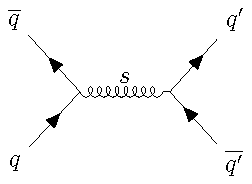
\includegraphics[width=2.5cm]{{img/DiagrammiPartonic/feynman_partonic_4.pdf}}}} & $\displaystyle{\frac{4}{9}\frac{t^2+u^2}{s^2}} $\\\hline
	$q\overline{q}\,\rightarrow\,q\overline{q} $ & \scalebox{0.95}{\raisebox{-.5\height}{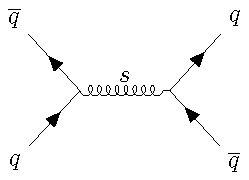
\includegraphics[width=2.5cm]{{img/DiagrammiPartonic/feynman_partonic_5.pdf}}\qquad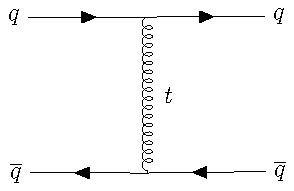
\includegraphics[width=2.5cm]{{img/DiagrammiPartonic/feynman_partonic_6.pdf}}}} & $\displaystyle{\frac{4}{9}\frac{s^2+u^2}{t^2} + \frac{4}{9}\frac{t^2+u^2}{s^2} - \frac{8}{27}\frac{u^2}{st}}$\\\hline
	$q\overline{q}\,\rightarrow\,gg $ & \scalebox{0.95}{\raisebox{0.0\height}{\vtop{\hbox{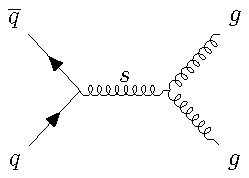
\includegraphics[width=2.5cm]{{img/DiagrammiPartonic/feynman_partonic_7.pdf}}\qquad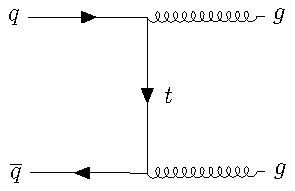
\includegraphics[width=2.5cm]{{img/DiagrammiPartonic/feynman_partonic_8.pdf}}}\begin{minipage}{4cm}{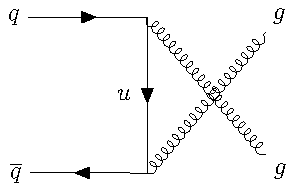
\includegraphics[width=2.5cm]{{img/DiagrammiPartonic/feynman_partonic_9.pdf}}}\end{minipage}}}} & $\displaystyle{\frac{32}{27}\frac{t^2+u^2}{tu}-\frac{8}{3}\frac{t^2+u^2}{s^2}} $\\\hline
	$gg\,\rightarrow\,q\overline{q} $ & \scalebox{0.95}{\raisebox{0.0\height}{\vtop{\hbox{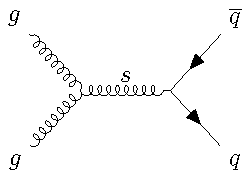
\includegraphics[width=2.5cm]{{img/DiagrammiPartonic/feynman_partonic_10.pdf}}\qquad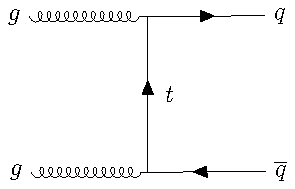
\includegraphics[width=2.5cm]{{img/DiagrammiPartonic/feynman_partonic_11.pdf}}}\begin{minipage}{4cm}{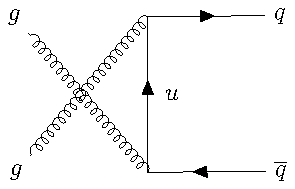
\includegraphics[width=2.5cm]{{img/DiagrammiPartonic/feynman_partonic_12.pdf}}}\end{minipage}}}} & $ \displaystyle{\frac{1}{6}\frac{t^2+u^2}{tu}-\frac{3}{8}\frac{t^2+u^2}{s^2}} $\\\hline
	$qg\,\rightarrow\,qg $ & \scalebox{0.95}{\raisebox{0.0\height}{\vtop{\hbox{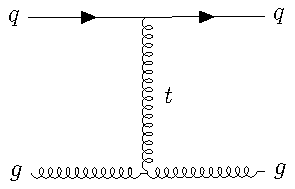
\includegraphics[width=2.5cm]{{img/DiagrammiPartonic/feynman_partonic_13.pdf}}\qquad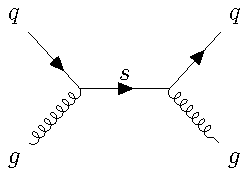
\includegraphics[width=2.5cm]{{img/DiagrammiPartonic/feynman_partonic_14.pdf}}}\begin{minipage}{4cm}{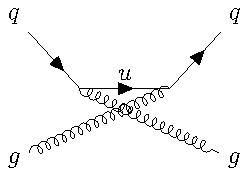
\includegraphics[width=2.5cm]{{img/DiagrammiPartonic/feynman_partonic_15.pdf}}}\end{minipage}}}} & $ \displaystyle{-\frac{4}{9}\frac{s^2+u^2}{su}+\frac{s^2+u^2}{t^2} }$\\\hline
	$gg\,\rightarrow\,gg $ & \scalebox{0.95}{\raisebox{0.1\height}{\vtop{\hbox{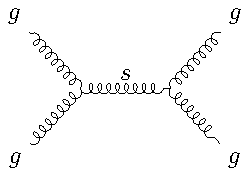
\includegraphics[width=2.5cm]{{img/DiagrammiPartonic/feynman_partonic_16.pdf}}\qquad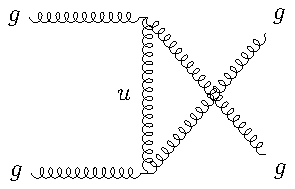
\includegraphics[width=2.5cm]{{img/DiagrammiPartonic/feynman_partonic_17.pdf}}}\hbox{\raisebox{0.1\height}{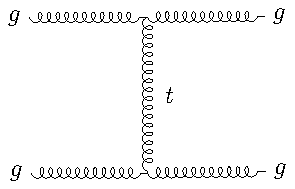
\includegraphics[width=2.5cm]{{img/DiagrammiPartonic/feynman_partonic_18.pdf}}\qquad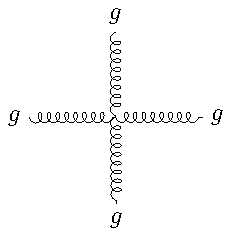
\includegraphics[width=2.5cm]{{img/DiagrammiPartonic/feynman_partonic_19.pdf}}}}}}} & $ \displaystyle{\frac{9}{2}\left( 3-\frac{tu}{s^2}-\frac{su}{t^2}-\frac{st}{u^2}\right)} $\\\hline
	\end{tabular}
	\caption{Parton-Parton differential cross-sections ($2\ \rightarrow\ 2$ QCD process), can beh calculated in pQCD by evaluating the matrix element for each process involving quark, antiquark and gluon. Table from \cite{SIEGERTthesis}}
	\label{table:partonic_cross_sections}
\end{table}

%\begin{table}[!ht]
%	\centering
%	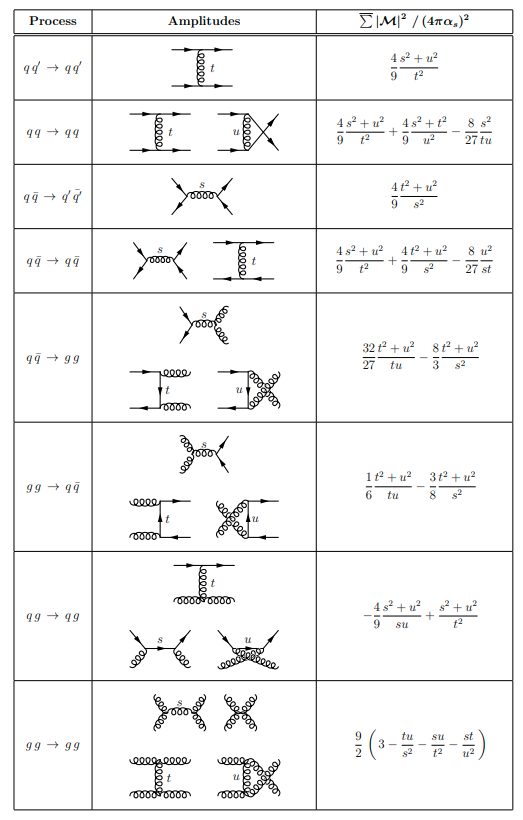
\includegraphics[width=0.8\textwidth]{{img/Table_cross_sections.png}}
%	\caption{Parton-Parton differential cross-sections ($2\ \rightarrow\ 2$ QCD process), can beh calculated in pQCD evaluating the matrix element for each process involving quark, antiquark and gluon. Table from \cite{SIEGERTthesis}}
%	\label{table:partonic_cross_sections}
%\end{table}

\noindent As one can see from the formulae in \tableRef{table:partonic_cross_sections}
at small scattering angles, for $t\,\rightarrow\,0$,  the t-channel gluon exchange processes $qq'\,\rightarrow\,qq'$, $qg\,\rightarrow\,qg$ and $gg\,\rightarrow\,gg$ dominate the full matrix element. For scatterings that are soft relative to $\hat{s}$, $|\hat{t}|\ll \hat{s}$, it is possible to approximate $|\hat{t}|$ as:
\begin{equation}
	p_T^2=\frac{\hat{t}\hat{u}}{\hat{s}} = \frac{\hat{t}(-\hat{s}-\hat{t})}{\hat{s}} \approx |\hat{t}|\quad ,
\end{equation}
in this limit, the only differences between quark and gluon cross-sections are the color factors.
\begin{equation}
	\hat{\sigma}_{gg}:\hat{\sigma}_{qg}:\hat{\sigma}_{qq}=\frac{9}{4}:1:\frac{4}{9}\quad .
\end{equation}
So, the \eqRef{eq:sigma_int1} can be rewritten like:
\begin{equation}
	\frac{d\sigma_{int}}{dp_T^2}\approx\int\int\frac{dx_1}{x_1}\,\frac{dx_2}{x_2}\,F(x_1,p_T^2)\,F(x_2,p_T^2)\frac{d\hat{\sigma}_{2\,\rightarrow\,2}}{dp_T^2}\quad ,
	\label{eq:sigma_int2}
\end{equation}
whit:
	\begin{gather}
		\frac{d\hat{\sigma}_{2\,\rightarrow\,2}}{dp_T^2} = \frac{8\pi\alpha_s^2(p_T^2)}{9p_T^4}\quad ;\\
		F(x,Q^2)=\displaystyle\sum_q\left( x\,q(x,Q^2) + x\,\overline{q}(x,Q^2) \right) + \frac{9}{4}\,x\,g(x,Q^2)\quad .
	\end{gather}
Now, the \eqRef{eq:sigma_int2} can be integrated:
\begin{equation}
	\sigma_{int}(p_{T\,min})= \displaystyle\int_{ p_{T\,min}^2}^{(\sqrt{s}/2)^2}\frac{d\hat{\sigma}_{2\,\rightarrow\,2}}{dp_T^2}\,dp_T^2\propto \frac{1}{p_{T\,min}^2}\  \xrightarrow{\ \ p_{T\,min}\,\rightarrow\, 0 \ }\ \ \infty\quad.
	\label{eq:interaction_crossSection}
\end{equation}

\begin{figure}[!ht]
	\centering
	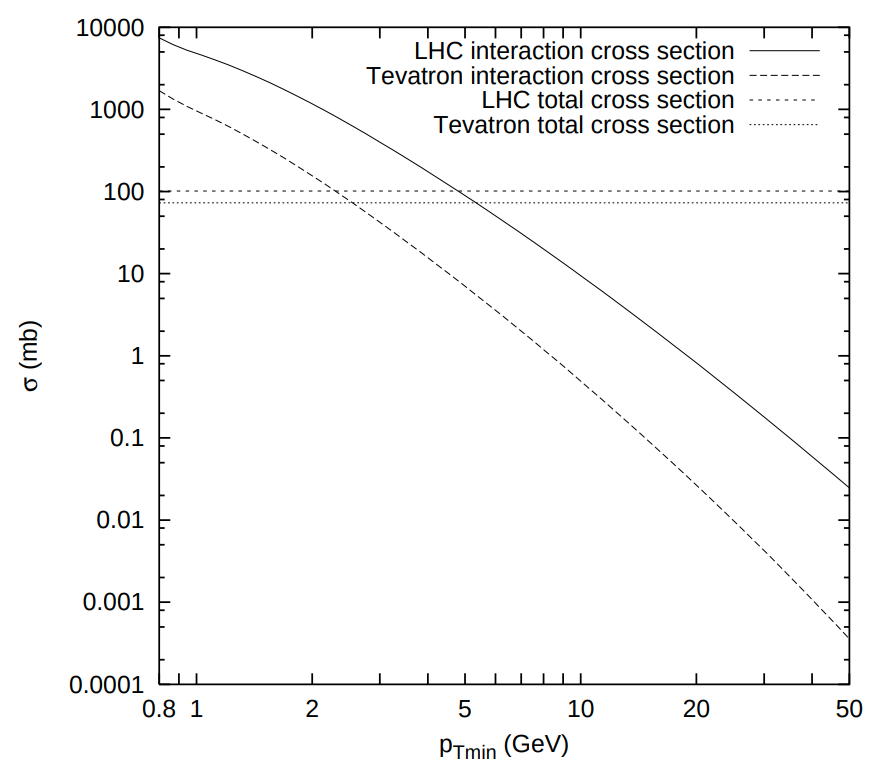
\includegraphics[width=12cm]{{img/CrossSection_Tot.png}}
	\caption{This figure shows the interaction cross-section ($\sigma_{\text{int}}$) at Tevatron ($p\overline{p}$, $\sqrt{s}=1.8\ \mathrm{TeV}$) and at LHC ($pp$, $\sqrt{s}=14\ \mathrm{TeV}$). The flat lines are the corresponding values for the total cross-section. The interaction cross-section that arise from \eqRef{eq:interaction_crossSection} is divergent for $p_{T\,min}\,\rightarrow\,0$ in reality a dumping of this divergence is expected due to the color screening effect.}
	\label{fig:CrossSection_Tot}
\end{figure}

\noindent The total cross-section is divergent in the limit $p_T\,\rightarrow\,0$. \figRef{fig:CrossSection_Tot} shows the rise of the interaction cross-section as the energy scale decreases. Due to this divergence, the total interaction cross-section at some $p_{T}$ scale can exceed the total proton-proton cross-section (described in the section above).
\\
To understand this paradox should be noted that the interaction cross-section described in \eqRef{eq:interaction_crossSection} is related to the interaction probability between two partons and counts the number of interactions, while the total proton-proton cross-section $\sigma_{pp}$ counts the number of events. For example, an event (a proton-proton collision) in which two partons interact counts once in the total cross-section and twice in the interaction cross-section.
\\
So, the ratio between these two quantities is perfectly allowed to be larger than unity, it can be written as:
\begin{equation}
	\frac{\sigma_{int}(p_{T\,min})}{\sigma_{tot}}=\langle n \rangle (p_{T\,min})\quad .
\end{equation}
Furthermore, the \textit{screening effect} has to be considered,  in fact, the incoming hadrons are color singlet objects but the partons are not. Therefore, when the $p_T$ of an exchanged gluon is small, and so the associated wavelength large, this gluon can no longer resolve the color charges and the effective coupling is decreased, this screening set a cutoff in the divergence. The screening effect is schematically shown in \figRef{fig:ScreeningEffect}.

\begin{figure}[!htb]
	\centering
	\noindent
	\begin{subfigure}{0.48\textwidth}
		\centering
		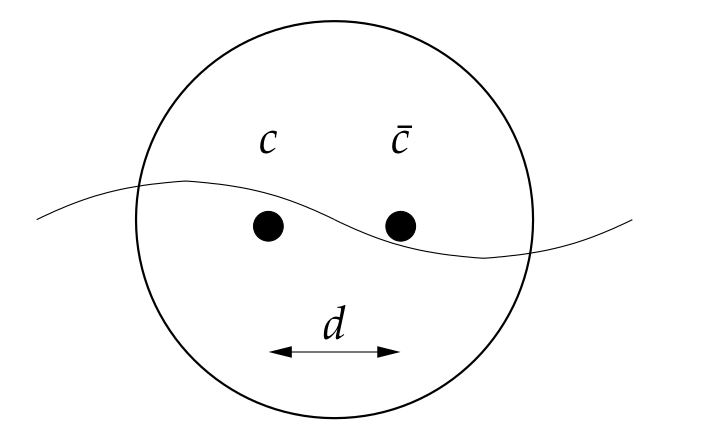
\includegraphics[width=0.8\textwidth]{{img/screening1.png}}
		\caption*{a) Screened color charges}
	\end{subfigure}%
	\begin{subfigure}{0.48\textwidth}
		\centering
		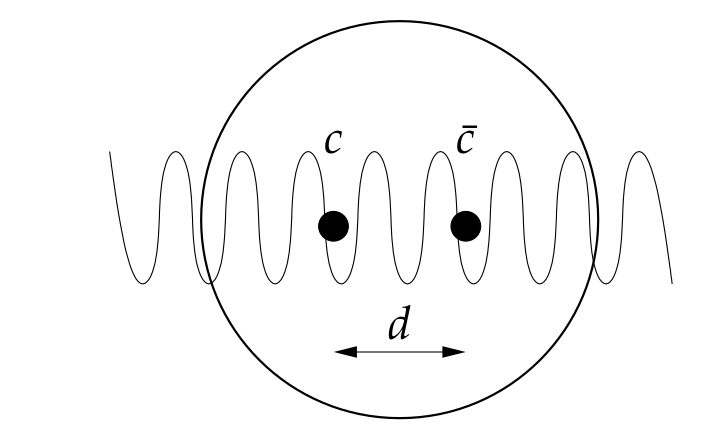
\includegraphics[width=0.8\textwidth]{{img/screening2.png}}
		\caption*{b) Resolved color charges}
	\end{subfigure}
	\caption{A picture of the screening effect. The left figure shows two color charges that are not resolved by the gluon in fact the wavelength is greater than the spatial separation, $d$, of the two charges. So the resolution of the probe is not enough to discriminate among the various color charges. While on the right figure the two charges are very well distinct.}
	\label{fig:ScreeningEffect}
\end{figure}

\noindent So, this cutoff is associated with color screening distance i.e. the average size of the region within which the  compensation of color charge occurs.
This cutoff is then introduced in the factor as:
\begin{equation}
	\frac{\alpha_s^2\,(p_{T0}^2+p_{T}^2)}{\alpha_s^2\,(p_T^2)}\,\frac{p_T^4}{(p_{T0}^2+p_T^2)^2}\quad .
\end{equation}
This factor contains the phenomenological regularization of the divergence, with the factor $p_{T0}$ that has to be tuned to data. 
\\
Now the interaction cross-section is smoothly regularized and therefore finite.
\\
To be notice that: parameter $p_{T0}$ does not have to be energy-independent, but since the energy is related to the sensitivity of the probe, higher energy is related to the capacity of probing PDFs to lower x values (as discussed previously, see \figRef{fig:NNPDF31}) and in this low-x region, the number of partons rapidly increases. So, the partons are more closely packed in this region and as a consequence the color-screening distance decrease.
\\
The number of partons is related to $x$ with a power-law so, it is likely to have a dependence of the same form for $p_{T0}$ with respect to the center-of-mass energy
\begin{equation}
	p_{T0}(\sqrt{s})=p_{T0}^{ref} \,\left( \frac{\sqrt{s}}{E_{CM}^{ref}} \right)^{E_{CM}^{pow}}\quad .
\end{equation}
%In the next section we are going to discuss how this and other effects fit into the Monte Carlo generator \textsc{pythia8}.	
These two parameters are named \texttt{MultiplepartonInteractions:}\-\texttt{pT0Ref} and \texttt{Mul}\-\texttt{tiple}\-\texttt{partonInteractions:}\-\texttt{ecmPow} and control respectively the threshold for the MPI to occur at a fixed center-of-mass energy and the power evolution with $\sqrt{s}$. 


In \textsc{pythia}8 MPI, as said before, are also generated in a decreasing $p_T$ sequence. So the hardest MPI is generated first. Then the probability for an interaction, $i$, to occur at a scale $p_T$ can be written using a Sudakov-type expression (as was done for the ISR and the FSR):
\begin{equation}
	\frac{d\mathcal{P}_{MPI}}{dp_T}=\frac{1}{\sigma_{ND}}\frac{d\sigma_{2\,\rightarrow\,2}}{dp_T}\ \exp\left( -\displaystyle\int_{p_T}^{p_T\,i-1} \frac{1}{\sigma_{ND}}\frac{d\sigma_{2\,\rightarrow\,2}}{dp_T'}\,dp_T' \right)\quad .
\end{equation}


\subsection{Momentum and flavour conservation}

One problem in MPI simulation is to achieve momentum conservation, so for every consecutive interaction, it has to be taken into account the modification in the PDFs by the preceding, $i-1$, interaction. To do that in \textsc{Pythia} the PDF are rescaled to the remaining available $x$ range, adjusting their normalization.
\\
One needs to take into account the momentum fraction $x_i$ removed from the hadron remnant by the $i-th$ interaction. This is done by evaluating PDF not at $x_i$ but at a rescaled value
\begin{equation}
	x_i'=\frac{x_i}{X} \qquad \ \text{with }\ \ X=1-\sum_{j=1}^{i-1}x_j\quad .
\end{equation}
So, by using these quantities, the PDFs can be rewritten as:
\begin{equation}
	f_i(x,Q^2)\ \longrightarrow\ \frac{1}{X}f_0\left(\frac{x}{X},Q^2\right)\quad ,
\end{equation}
where $f_0$ is the original one-parton inclusive PDFs.
\\
Now, requiring also the flavour conservation and taking into account the number of valence and/or sea quarks involved in the preceding MPI. The full forms of the PDFs used for the $i-th$ MPI are:
\begin{align}
f_i(x,Q^2) =&  \frac{N_{fv}}{N_{fv0}}\frac{1}{X} f_{v0}\left( \frac{x}{X},Q^2 \right) + \frac{a}{X}f_{s0}\left( \frac{x}{X},Q^2 \right)+\displaystyle\sum_j \frac{1}{X} f_{c_j0}\left( \frac{x}{X},Q^2 \right) \quad,\\
g_i(x,Q^2) =& \frac{a}{X}g_0\left( \frac{x}{X},Q^2 \right)\quad, 
\end{align}
where: 
\begin{itemize}
	\item $f_i(x,Q^2)$ $(g_i(x,Q^2))$ are the squeezed PDFs for quarks (gluons);
	\item $N_{fv}$ the number of remaining valence quarks of the given flavour;
	\item $N_{fv0}$ the number of original valence quarks of the given flavour (for the proton they are: $N_u=2$, $N_d=1$);
	\item $f_{s0}$ the sea-quark PDF;
	\item $f_{cj}$ the companion PDF, this arise from the splitting $g\,\rightarrow\,q\overline{q}$ and a quark $j$ is kicked out.
\end{itemize}
The factor $a$ is defined to satisfy the total momentum sum rule.

\subsection{Impact Parameter Dependence}

The simplest hypothesis for the multiple interaction simulation is to assume the same initial state for all hadron collisions without dependencies on the impact parameter. 
\\
The more realistic scenario is to include the possibility that each collision could be characterized by a different impact parameter $b$, where a small $b$ value corresponds to a large overlap between the two hadrons this is related to the probability of parton-parton interaction to take place.
\\
To include the impact parameter dependence on the collision, it is necessary to make some assumptions on the matter distribution inside the proton. A possibility is to assume a spherically symmetric distribution inside an hadron at rest $\rho(\mathbf{x})\,d^3x=\rho(r)\,d^3x$. A Gaussian ansatz is the most simple choice but it appears to lead to a narrow multiplicity distribution and a too little pedestal effect. So the choice is a double Gaussian:
\begin{equation}
	\rho(r) \propto \frac{1-\beta}{a_1^3}\exp\left\{-\frac{r^2}{a_1^2}\right\}+\frac{\beta}{a_2^3}\exp\left\{ -\frac{r^2}{a_2^2} \right\}\quad,
	\label{eq:matterDistribution}
\end{equation}
where a fraction $\beta$ of matter is contained in a smaller central region, called \textit{core}, of radius $a_2$, while the rest of the matter fraction in a larger one of radius $a_1$. In \textsc{pythia8} the two parameters related to the fraction of matter and the spatial extension of the core region are named respectively as \texttt{Multiparton}\-\texttt{Interactions:}\-\texttt{core}\-\texttt{Fraction} and \texttt{Multiparton}\-\texttt{Interactions:}\-\texttt{core}\-\texttt{Radius}.
\\
Now, for a given matter distribution $\rho(r)$,  the time-integrated overlap function of the incoming hadrons during the collision is given by:
\begin{equation}
	\mathcal{O}(b)=\displaystyle\int dt \displaystyle\int d^3x\,\rho(x,y,z)\,\rho(x+b,y,z+t)\quad.
	\label{eq:overlappingFunction}
\end{equation} 
Assuming the matter distribution function in \eqRef{eq:matterDistribution} and inserting it into \eqRef{eq:overlappingFunction}, one obtains the following expression:
\begin{equation}
\small{
	\mathcal{O}(b)\propto \frac{(1-\beta)^2}{2a_1^2}\exp\left\{-\frac{b^2}{2a_1^2}\right\}+\frac{2\beta(1-\beta)}{a_1^2+a_2^2}\exp\left\{ -\frac{b^2}{a_1^2+a_2^2} \right\}+\frac{\beta^2}{2a_2^2}\exp\left\{-\frac{b^2}{2a_2^2}\right\}
	}
\end{equation}
This quantity is useful to quantify the effect of overlapping protons.
The larger is $\mathcal{O}(b)$ the more probable are parton-parton scatters between the incoming protons. So, it is natural to assume a linear relationship between the overlapping function and the mean number of interactions in the event as in the following equation: 
\begin{equation}
\langle \widetilde{n} \rangle = k \mathcal{O}(b)\quad.
\end{equation}
In this scenario, the number of interactions at a fixed impact parameter value is given by a Poissonian distribution:
\begin{equation}
\mathcal{P}(\widetilde{n})=
	\left\langle \widetilde{n}\right\rangle ^{\widetilde{n}}\ \frac{e^{-\langle\widetilde{n}\rangle}}{\widetilde{n}!}
	\label{eq:poisson}
\end{equation} 

%So, these assumption change the so-far Poissonian nature of the framework\footnote{the Poissonian distribution, in \eqRef{eq:poisson} describe the probability of having $n$ interactions at each impact parameter. If the matter distribution have an infinite tail (like our in \eqRef{eq:matterDistribution}) events may be obtained with arbitrarily large b values. This can be a problem for the definition of the total hadron-hadron cross-section}
%\begin{equation}
%\mathcal{P}(\widetilde{n})=
%	\left\langle \widetilde{n}\right\rangle ^{\widetilde{n}}\ \frac{e^{-\langle\widetilde{n}\rangle}}{\widetilde{n}!}
%	\label{eq:poisson}
%\end{equation}
If the matter distribution has an infinite tail (like the one in \eqRef{eq:matterDistribution}) events may be obtained with arbitrarily large $b$ values. This can be a problem for the definition of the total hadron-hadron cross-section.
\\
So, imposing that at least one parton interaction occurs in the hadron-hadron collision, it is ensured that a finite total cross-section is obtained. The probability that at least one interaction occurs by a hadron scattering with impact parameter $b$  is:
\begin{equation}
	\mathcal{P}_{\text{int}}= \displaystyle\sum_{\widetilde{n}=1}^\infty\mathcal{P}_{\widetilde{n}(b)}=1-\mathcal{P}_0=1-e^{-\langle \widetilde{n}(b) \rangle}=1-e^{-k\mathcal{O}(b)}
\end{equation}
Now, the number of interaction, for impact parameter $b$, per event is give by:
\begin{equation}
	\langle \widetilde{n}(b) \rangle =\frac{\langle k\mathcal{O}(b) \rangle}{ 1-e^{-k\mathcal{O}(b)} } =\frac{\langle k\mathcal{O}(b) \rangle}{\mathcal{P}_{\text{int}}(b)}
\end{equation}
where it has been divided for the total interaction probability to take into account for the request of at least one parton interaction.
So, this have modified the probability distribution of interactions number from a Poissonian to a narrower one at each $b$ fixed.

\subsection{Parton rescattering}

It is not necessary that the partons undergoing MPI are a different partons couple from the one scattered before. As shown in \figRef{fig:Rescattering} MPI can also arise when a parton scatters more than once against partons from the other beam, this is called \textit{parton rescattering}.
%
\begin{figure}[!htb]
	\centering
	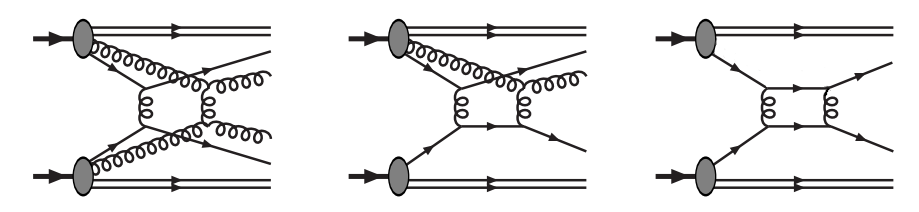
\includegraphics[width=0.95\textwidth]{{img/Rescattering_3casi.png}}
	\caption{This figure shows parton rescattering. On the left image a double $2\,\rightarrow\,2$ scattering (no rescattering) is shown; on the middle a parton rescattering process where only one of the rescattered partons has already scattered; on the right image a parton rescattering with both the partons that undergo to rescattering have already been scattered. }
	\label{fig:Rescattering}
\end{figure}
%

\noindent MPI can take place in three different ways:
\begin{enumerate}
	\item No one of the partons that enter in the second scattering undergoes to another scatter before (\figRef{fig:Rescattering} left);
	\item Only one of the two partons has already been scattered (\figRef{fig:Rescattering} middle); In very rough terms, this means that the non-diffractive
cross-section is saturated by more than a single partonic scattering and that the number of partonic
interactions is determined by a Poisson distribution. This model, which was originally proposed in [98]
has been very successful in the description of many experimental measurements at hadron colliders.
	\item Both the partons have already been scattered before (\figRef{fig:Rescattering} right). 
\end{enumerate}
The second and the third are the rescatters. The overall influence of rescatters in proton-proton interactions was estimated to be small with respect to the first case with distinct $2\,\rightarrow\,2$  scatters. 
\\
The simulation of partons rescattering starts from the evaluation of the parton density as:
\begin{equation}
	f(x,Q^2)\ \  \longrightarrow\! \underbrace{\phantom{\Bigg(} f_{\text{rescaled}}(x,Q^2)}_{\text{hadron remnant}}+\underbrace{\displaystyle\sum_{i=1}^N \,\delta(x-x_i)}_{\text{scattered parton(s)}}\quad,
\end{equation} 
where the $\delta(x-x_i)$ takes into account the $N$  already-scattered partons that have a fixed momentum fraction $x_i$. While the hadron remnants that do not enter a scattering before are still described by a continuous momentum density, but re-scaled to achieve momentum conservation once that the already-scattered partons have been extracted:
\begin{equation}	\displaystyle\int_0^1 \bigg( f_{\text{rescaled}}(x,Q^2) +\displaystyle\sum_n \,\delta(x-x_n) \bigg)dx=1\quad.
\end{equation}


\subsection{Interplay of Multiple Interaction and Parton Shower}

%As discussed above the ISR, FSR and MPI are simulated in \textsc{Pythia} following a common decreasing $p_T$ evolution.
Obviously, the parton shower can be applied not only to the partons that undergo to the primary hard scattering, but also the other partons especially the ones interested by the MPI. 
\\
In other words, the event structure of a hadron-hadron collision can be very complex, e.g. a single initial-state parton can split into two before both of them enter a hard collision. At the same time, an independently resolved parton may undergo another collision, while all of them collectively radiate further gluons. This is a very complex situation that cannot be described exactly. But a good description can be obtained by considering an \textit{interleaved} parton shower and MPI evolution. An example of a possible resulting event structure is reported in \figRef{fig:PartonShower}.
\\
The total interaction probability is given from the composition of the various contributions from each process:
\begin{align}
	\frac{d\mathcal{P}}{dp_T}=&\left( \frac{d\mathcal{P}_{MPI}}{dp_T}+\displaystyle\sum\frac{d\mathcal{P}_{ISR}}{dp_T}+\displaystyle\sum\frac{d\mathcal{P}_{FSR}}{dp_T} \right) \nonumber \times\\ 
	&\times\exp\left\{ -\displaystyle\int_{p_T}^{p_T\,i-1} \left( \frac{d\mathcal{P}_{MPI}}{dp_T'}+\displaystyle\sum\frac{d\mathcal{P}_{ISR}}{dp_T'}+\displaystyle\sum\frac{d\mathcal{P}_{FSR}}{dp_T'} \right)\,dp_T' \right\}
	\label{eq:common_pT_sequence}
\end{align}
%
\begin{figure}[!htb]
	\centering
	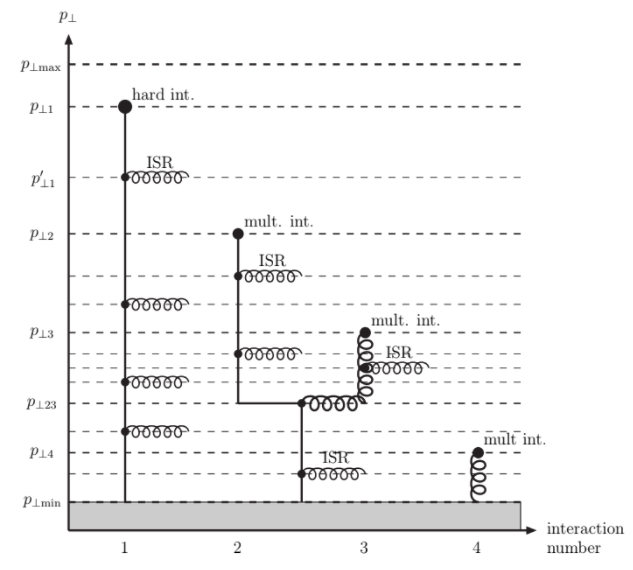
\includegraphics[width=12cm]{{img/PartonShower.png}}
	\caption{An example of Multiple Partons Interactions and associated radiations. The downward evolution in $p_T$ is shown here by reading the graph from top to bottom. The 4 parton-parton interactions occur to $p_{T1}$, $p_{T2}$, $p_{T3}$ and $p_{T4}$.}
	\label{fig:PartonShower}
\end{figure}
%
\\
In \figRef{fig:PartonShower} are shown 4 parton-parton interactions with their associated showers (ISR and FSR). The downward evolution correspond to read the graph from top to bottom. The first hard interaction occurs at a scale $p_T=p_{T1}$ while the following ones at lower scales $p_{T2}$, $p_{T3}$, $p_{T4}$. Each interaction is associated with is radiation the first one occurs at $p_T=p_{T1}'$.
The scatterings at $p_{T2}$ and $p_{T3}$ are originating from the same mother parton. 
\\
This diagram is related to one of the two hadrons. The full event can be illustrated if a similar diagram is drawn for the other hadron and connected to the full black circles.


\section{Primordial $k_T$ and Color reconnection in PYTHIA8}
\label{sec:Beam Beam Remnants and primordial kT}

What is left after that the $p_T$ evolution is ended?
The evolution in $p_T$ can create an arbitrary complicated final state. 
This final state contains contributions from the scattered and unscattered partons that don't enter the $p_T$ evolution. The last ones are the so-called \textit{Beam Beam Remnants}. 
BBR take into account the number of valence quarks remaining and the number of sea quarks required for the overall flavour conservation and, to ensure momentum conservation. So, once the evolution ended, a set of partons is added to the BBR. The BBR have to take all the remaining longitudinal momentum that is not extracted by the MPI initiators to ensure the overall momentum conservation.
\\
The showering process plus the MPI introduction lead to a large number of partons in the final states. Then, in the simulation, all the partons take the contribution from the primordial $k_T$ (originating from the Fermi motion) this is described in the next section.    

\subsection*{Primordial $k_T$}

It has been considered only the longitudinal momentum. In a real scenario partons, inside the hadrons, are fermions. So, are expected to have a non-zero initial transverse momentum arising from the Fermi motion inside the incoming hadrons. This is denoted as \textit{primordial $k_T$}. This is different from the transverse momentum derived from DGLAP shower evolution or from the hard interaction. 

\bigskip

\noindent Based on Fermi motion alone, one would expect a value of the primordial $k_T$ of the order of the inverse hadron radius: 
\begin{equation}
	k_T\simeq\frac{\hbar}{r_p}\approx\frac{0.2\ \mathrm{GeV\cdot fm}}{0.7\ \mathrm{fm}}\approx0.3\ \mathrm{GeV}\quad,
\label{eq:PrimordialKT}
\end{equation}
but, as an example, to reproduce the data for the $p_T$ distributions of $Z$ bosons produced in hadron-hadron collisions and observed in Drell Yan processes, one needs a larger contribution from the primordial $k_T$. This phenomenon has not a satisfactory phenomenological explanation. Until a convincing explanation is found the idea is to consider an effective primordial $k_T$ for the initiators larger than the one in \eqRef{eq:PrimordialKT}. This larger value can be seen as a value re-summing also all the low-$p_T$ "unresolved" effects that are not taken into account by the showering and all the above processes.  

\medskip

In \textsc{pythia} the primordial kT is assigned to all shower initiators sampling a Gaussian distributions for $p_x$ and $p_y$ independently with variable width $\sigma$
\begin{equation}
	\sigma(Q,\widehat{m})=\frac{Q_{1/2}\,\sigma_{\text{soft}}+Q\,\sigma_{\text{soft}}}{Q_{1/2}+Q}\,\frac{\widehat{m}}{\widehat{m}_{1/2}+\widehat{m}}
\end{equation}
Where $Q$ is the hard-process renormalization scale for the main hard process and the $p_T$ scale for subsequent MPI. $\sigma_{\text{soft}}$, $\sigma_{\text{hard}}$ are the minimum and maximum width, $\widehat{m}$ is the invariant mass, while $Q_{1/2}$ and $\widehat{m}_{1/2}$ the halfway values between the two extremes.
\\
In \textsc{pythia} the maximum width parameters is called \texttt{Beam}\-\texttt{Remnants:}\-\texttt{primordialKT}\-\texttt{hard}.
\\
Note that in \textsc{pythia8} simulation the addition of the primordial kT to all shower initiators does not automatically guarantee overall $p_T$ conservation. To minimize the mismatch lot of tricks are used in the generator, and as the final step, a brute force shift is imposed on all the final state particles. 

\subsection{Color Reconnection}

The last important step at parton level is the \textit{color reconnection}. CR is motivated by the fact that MPI leads to different color strings. In the previous steps, the planar limit of the QCD was assumed where $N_c\rightarrow\infty$. Now, moving to real case where $N_c=3$  during the development of the parton shower, partons are
represented and also connected by colour lines as it is shown in \figRef{fig:CRrecon}. Quark and anti-quarks are described by a single color line with an arrow that describes the direction of the color flow, while gluons are represented by a pair of color lines pointing in opposite directions. 

\begin{figure}[!htb]
	\centering
	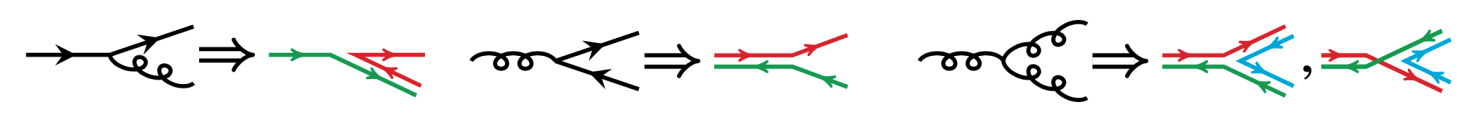
\includegraphics[width=0.95\textwidth]{{img/CRrecon.png}}
	\caption{Color flow in quark-gluon vertices. The Feynman diagrams are shown in black and associated with the respective color connection lines. This figure is taken from \cite{CRrecon}.}
	\label{fig:CRrecon}
\end{figure}

\noindent All these color strings that can be overlapped in physical space can be reconnected.  
The basic idea is to reconnect strings in order to reduce the total string length, and thus the potential energy (Lund Model).
\\
In \textsc{pythia8} different models for the CR exist. In the default model (\textit{MPI-based model}) the partons are classified according to the MPI system to which they belong\footnote{Note that each parton interaction is originally a $2\,\rightarrow\,2$ scattering. Further details on various models can be found at  \cite{CRrecon}.}, the  reconnection is performed giving to each system, whit a hardness scale $p_T$, a probability to reconnect defined by:
\begin{equation}
	\mathcal{P}_{\text{rec}}=\frac{p_{T\,\text{rec}}^2}{\left(p_{T\,\text{rec}}^2 + p_T^2\right)} \qquad\quad p_{T\,\text{rec}}=R\times p_{T\,0}\quad,
\end{equation} 
the \texttt{ColorReconnection:range}, $R$, is a user-tunable parameter while $p_{T\,0}$ is the same parameter defined in MPI simulation.
\\
With this definition for the probability, it is clear that systems with low $p_T$ are more likely to reconnect to others, while the higher-$p_T$ systems tend to escape from the interaction point without being reconnected. This idea finds its justification in the fact that lower $p_T$ values correspond to larger spatial extension and so these strings have more chance to overlap with others and so the systems to reconnect.

\section{Hadronization}


The hadronization process takes all these partons (colored strings) and transforms them into a set of experimental-observed color-neutral hadrons. 
\\
Hadronization is one of the most non-understood process in high energy physics. Due to the intrinsically non-perturbative nature of the phenomenon, it cannot be derived by QCD fundamental principles. A good description of the hadronization is needed it participate in all the interaction that contain a final-state composed of colored partons. So, necessarily, the simulated final-state depends strongly on the hadronization model used.  
\\
There are two main hadronization model classes in current use: the \textit{string} and the \textit{cluster model}. \textsc{pythia8} is based on the former. the following will describe the string model.

\subsection{String model}

In Pythia hadronization is based solely on the \textit{Lund string fragmentation model} \cite{ANDERSSON198331, Sjostrand:1984ic}. 
\\
The Lund model's basic idea is to break the color lines that connect the quarks to reduce the total string length, where the string is representative of the potential:
\begin{equation}
	V(r)=-\frac{a}{r}+\kappa r \qquad\qquad \text{with}\quad \kappa\approx1\ \mathrm{GeV/fm}\quad,
\end{equation}
where $\kappa$ is the string tension.  This potential is a combination of an attractive (Coulomb) potential and of a linear potential that phenomenologically includes quarks confinement expected in QCD. The linear potential is the dominating part at increasing distance values, so the energy increase with distance. 
\\
The simplest case is the one in \figRef{fig:StringBreakings}: the back-to-back production of a $q\overline{q}$ pair. The $q\overline{q}$ system evolves in space increasing the string length at some point the distance is too large and is convenient to break the string into two shorter strings.

\begin{figure}[!htb]
	\centering
	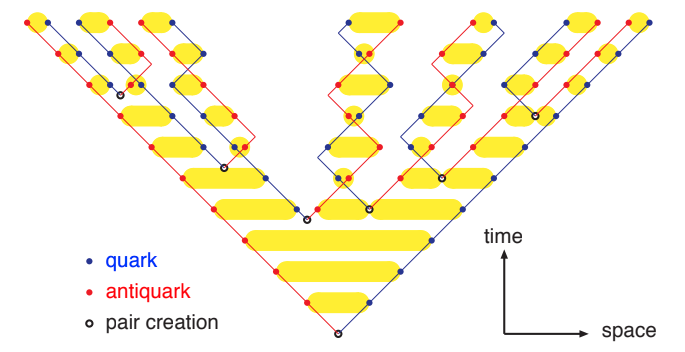
\includegraphics[width=12cm]{{img/StringBreakings.png}}
	\caption{The Lund Model is schematically shown here. The string evolution in time is shown vertically, while the spatial position is displayed horizontally. As the partons move apart at some point becomes convenient to break the string, in order to reduce the total potential energy, and a partons pair is produced.}
	\label{fig:StringBreakings}
\end{figure}

%So the hadronization try to reduce the string length.
\begin{equation}
	V(r)=-\frac{a}{r}+\kappa r \qquad\qquad \text{with}\quad \kappa\approx1\ \mathrm{GeV/fm}
\end{equation}
The hadronization step confines the quark into hadrons, then these hadrons can undergo to hadron rescattering and decay. These are the hadrons that are revealed by the detectors.

\section{\textsc{pythia} summary}


To summarize \textsc{pythia8} is a standard tool in high energy physics studies. It is able to simulate high energy hadron-hadron collisions showing a good agreement on lots of studied distributions in the past. 
\\
The simulation starts from a hard scattering calculated perturbatively at a fixed order using matrix elements calculations. Once the hard scattering has been simulated the parton showering process takes place on all the incoming (ISR) and outgoing (FSR) partons that enter the main hard scattering. 
\\
Additionally, by the fact that hadrons are composite objects, also extra parton scatterings can occur. They are named MPI. The interplay between MPI and parton shower can be really complicated in a real collision. In \textsc{pythia}, to achieve a good description of these complex situations the MPI, ISR and FSR are described in a common sequence of decreasing $p_T$ starting at the hardest scale defined by the hard interaction and proceeding downward until a cutoff value, $p_{T\,0}$ is reached.
\\
The interleaving of MPI and parton shower creates a very complex final-state of colored partons.
To this final-state is then added the contribution from the primordial $k_T$.
Moving to the real QCD case where the number of the possible charges of color is $N_C=3$ all these colored strings, created in the previous steps, may overlap in the physical space and then reconnect each other, merging the lower-$p_T$ MPI systems to the ones in higher-$p_T$ MPI.   
\\
This was the last step at the partonic level simulated by \textsc{pythia}, then the hadronization process, based on the Lund string fragmentation model takes place and transforms the partonic-state into a set of hadrons. Moreover, this hadron can undergo to hadron rescattering and decays before the detection.


%To summarize \textsc{pythia8} is able to simulate high energy hadron-hadron collisions. The evolution of the system is simulated in a common decreasing-$p_T$ sequence in order to achieve the master formula for the evolution is written in \eqRef{eq:common_pT_sequence}. 
%\\
%This evolution start from an hard scale that is the scale of the main parton hard scattering that is described by a fixed ME calculation, \textsc{pythia} can be interfaced with external frameworks for the ME step as \textsc{powheg} and \textsc{mad-graph5 amc@nlo} (some care have to be taken as described in \secRef{sec:merging}). Then the parton shower is started with the simulation of ISR, FSR and MPI also the parton rescattering is allowed. Once the evolution is ended the color reconnection and the hadronization transform the partons in a set of final hadrons these hadron than decay and rescatters against each others before the detection.
%\\
%A schematic view of these processes is shown in \figRef{fig:Processes}.
%
%\begin{figure}[!htb]
%	\centering
%	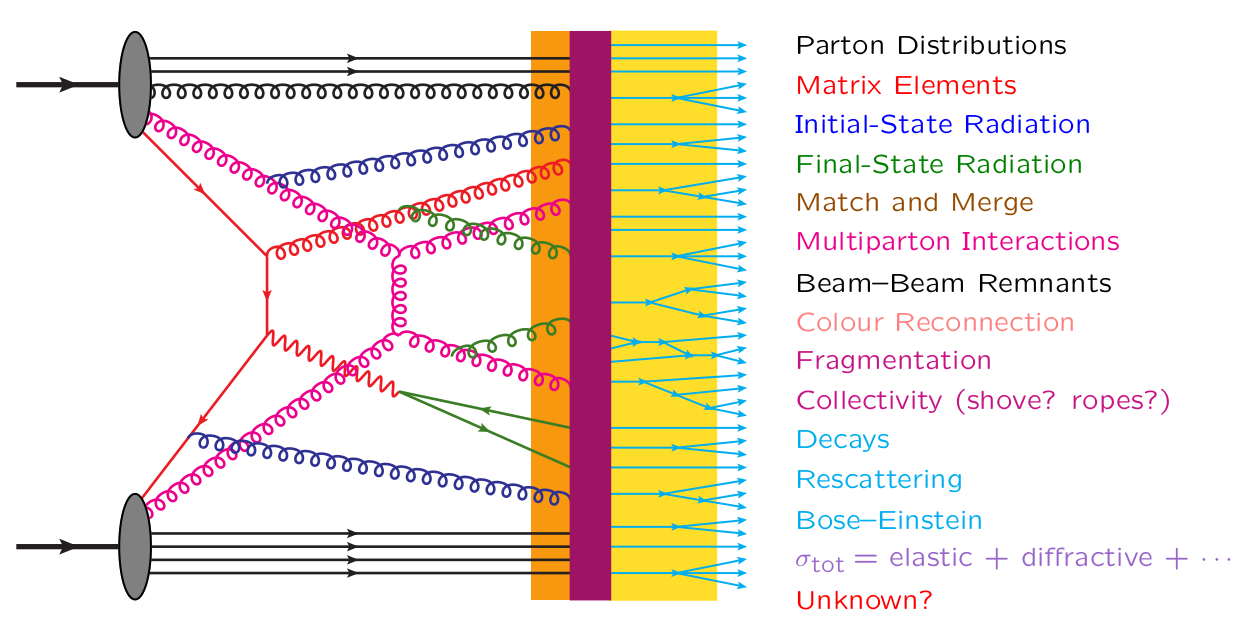
\includegraphics[width=0.98\textwidth]{{img/Processes.png}}
%	\caption{A schematic representation for a $pp$ collision. Reading the image from left to right one can have an idea on the evolution of the system. The two incoming hadrons enter the scattering from the left side, the red line indicate the main hard scattering and the magenta one the second parton scattering (MPI) each interaction is associated with initial (blue) and final (green) state radiation, the unscattered partons (black lines) re-enter the color reconnection and hadronization processes. Than the new formed hadrons (lightblue) can undergo to different decays.}
%	\label{fig:Processes}
%\end{figure}


\noindent All these processes simulated by \textsc{pythia} are described mainly by phenomenological models, due to the not-known-by-first-principles soft QCD description. The use of these phenomenological models introduces lots of free parameters (some are been pointed out in these sections) that have to be tuned with data to give  \textsc{pythia} the ability to reproduce real data observed experiments. The simulation is necessary to understand the observables histograms that are collected at colliders experiments in particular for the study of the UE.  

\section{Validation and tuning of a Monte Carlo generator}

Validating a Monte Carlo generator means to confront a model with all the relevant data that it claims to be able to describe. It is really important that the validation of the MC generator is global if one wants a predictive power from this generator. Otherwise, the generator is just parameterizing the data and not simulating the UE. 
\\
The validation is important for developing new models and debugging physics models. 
Tuning the generator refers to the operation of adjusting the parameters of the generator to improve the description of the relevant data.
\\
To perform both the validation and the tune of the generator a range of observables have to be simulated and analyzed. The various tuning computational procedure used for the optimization over the possible space of parameters are better described in \chapRef{chap:TuneprocedureCP5TuneandMCNNTUNES}.
\\
A general-purpose event generator contains a lot of parameters and so the parameter space to investigate is too large, it is impossible to investigate it in a comprehensive way. The strategy is to factorize the parameters into different sets based on the group of observables has been found to be important.
\\
So, usually, the tuning of the generators proceeds in consecutive steps:
\begin{itemize}
	\item \textit{Hadronization and final-state:} This step is performed employing data from $e^+e^-$ colliders. In fact, these observables are not sensible to initial-state hadron effects. So, the typical parameters tuned in this type of event are the $\alpha_s^{FSR}$ value, the cutoff of the FSR and the parameters related to the hadronization process: the string tension and the fragmentation functions.
	\item \textit{initial-state shower:} Parameters related to final-state effects have been fixed. Now, the initial-state ones are investigated, typically in observables of jet shapes. The analysis of these parameters is performed before the analysis of the MPI-related ones. In this way, it is avoided the risk of absorbing effects which should be perturbatively describable into the MPI modeling. The parameters tuned in this phase are the cutoff for the ISR, the $\alpha_s^{ISR}$ value and others related to the initial-state effects.
	\item \textit{MPI and BBR:} The parameters related to the MPI and BBR are the last tuned because they are the less constrained by the QCD calculation and have lots of free parameters that absorb all the non-perturbative effects.  
The typical observables for MPI and BBR tuning  are underlying event data from various hadron colliders. 	
\end{itemize}
This thesis focus on this last step. The next chapter will focus on the study of the underlying event with the description of all the distributions used in the tune and the effects of some of these \textsc{pythia}8 parameters on these observable distributions. 

The histograms of the observables useful for testing the physics of the MC generator are encoded in the tool: \textit{Rivet} \cite{RivetPaiper}.

\subsection{Rivet and Yoda format}

Rivet is a Monte Carlo event generator validation tool. It provides a large set of experimental analyses that can be used for the development, validation and tuning of event generators. Rivet structure contains different layers. A C++ shared library is the core, it is supplemented by C++ "plugin" libraries containing collider analysis routines. Then a Python programming interface  and a set of Python and shell scripts are the interfaces to it. 

The MC simulated events are passed into rivet that, thanks to the I/O interface based on \textsc{HepMC} \cite{HepMC} and \textsc{yoda} \cite{YODA} libraries, perform the analysis and organize them into histograms that are saved into the \textsc{yoda} format. The set of the Rivet instruction to perform the analysis are usually referred to as "routine".

These \textsc{yoda} files are the input format for the tools used for the tune of MC event generators: \textsc{professor} \cite{Buckley:2009bj} and \textsc{mcnntunes} \cite{MCNNTUNESarticle}.
